% Options for packages loaded elsewhere
\PassOptionsToPackage{unicode}{hyperref}
\PassOptionsToPackage{hyphens}{url}
\PassOptionsToPackage{dvipsnames,svgnames,x11names}{xcolor}
%
\RequirePackage[l2tabu,orthodox]{nag}
\documentclass[%
	12pt,
		oneside,
		letterpaper
]{book}

\usepackage{amsmath,amssymb}
\usepackage{iftex}
\ifPDFTeX
  \usepackage[T1]{fontenc}
  \usepackage[utf8]{inputenc}
  \usepackage{textcomp} % provide euro and other symbols
\else % if luatex or xetex
  \usepackage{unicode-math}
  \defaultfontfeatures{Scale=MatchLowercase}
  \defaultfontfeatures[\rmfamily]{Ligatures=TeX,Scale=1}
\fi
\usepackage{lmodern}
\ifPDFTeX\else  
    % xetex/luatex font selection
\fi
% Use upquote if available, for straight quotes in verbatim environments
\IfFileExists{upquote.sty}{\usepackage{upquote}}{}
\IfFileExists{microtype.sty}{% use microtype if available
  \usepackage[]{microtype}
  \UseMicrotypeSet[protrusion]{basicmath} % disable protrusion for tt fonts
}{}
\usepackage{xcolor}
\setlength{\emergencystretch}{3em} % prevent overfull lines
\setcounter{secnumdepth}{5}


\providecommand{\tightlist}{%
  \setlength{\itemsep}{0pt}\setlength{\parskip}{0pt}}\usepackage{longtable,booktabs,array}
\usepackage{calc} % for calculating minipage widths
% Correct order of tables after \paragraph or \subparagraph
\usepackage{etoolbox}
\makeatletter
\patchcmd\longtable{\par}{\if@noskipsec\mbox{}\fi\par}{}{}
\makeatother
% Allow footnotes in longtable head/foot
\IfFileExists{footnotehyper.sty}{\usepackage{footnotehyper}}{\usepackage{footnote}}
\makesavenoteenv{longtable}
\usepackage{graphicx}
\makeatletter
\newsavebox\pandoc@box
\newcommand*\pandocbounded[1]{% scales image to fit in text height/width
  \sbox\pandoc@box{#1}%
  \Gscale@div\@tempa{\textheight}{\dimexpr\ht\pandoc@box+\dp\pandoc@box\relax}%
  \Gscale@div\@tempb{\linewidth}{\wd\pandoc@box}%
  \ifdim\@tempb\p@<\@tempa\p@\let\@tempa\@tempb\fi% select the smaller of both
  \ifdim\@tempa\p@<\p@\scalebox{\@tempa}{\usebox\pandoc@box}%
  \else\usebox{\pandoc@box}%
  \fi%
}
% Set default figure placement to htbp
\def\fps@figure{htbp}
\makeatother

\directlua{pdf.setminorversion(6)}
\usepackage[T1]{fontenc}
\usepackage[utf8]{inputenc}

\usepackage[english]{babel}
\usepackage[strict]{csquotes}

% Change contents title to Table of Contents
\addto\captionsenglish{% Replace "english" with the language you use
  \renewcommand{\contentsname}%
    {Table of contents}%
}

% Bibliography
\usepackage[%
	backend=biber,
	style=ieee, % pick whatever style you want
	sorting=ydnt,
	isbn=true,
]{biblatex}
\addbibresource{bibliography.bib}

% Line spacing
\usepackage{setspace}

\usepackage{etoolbox}

\usepackage[unicode=false]{hyperref}

% \usepackage[notbib,notindex]{tocbibind}

\usepackage[%
	%textwidth=345pt, % Default textwidth
	% marginpar=4cm, % Make marginal notes wider
	% includemp, % Include marginpar in width
	margin=1in,
	left=1.5in, % Left margin must be at least 1.5 inch
]{geometry}

% Toggle for double spaced or not
% \newbool{doublespaced}
\usepackage{titlesec}
   
\titleformat{\chapter}[block]{\normalfont\large}{Chapter \ \thechapter:}{1em}{}[]
\titleformat{\section}{\normalfont\large}{\thesection}{1em}{}
\makeatletter
\@ifpackageloaded{bookmark}{}{\usepackage{bookmark}}
\makeatother
\makeatletter
\@ifpackageloaded{caption}{}{\usepackage{caption}}
\AtBeginDocument{%
\ifdefined\contentsname
  \renewcommand*\contentsname{Table of contents}
\else
  \newcommand\contentsname{Table of contents}
\fi
\ifdefined\listfigurename
  \renewcommand*\listfigurename{List of Figures}
\else
  \newcommand\listfigurename{List of Figures}
\fi
\ifdefined\listtablename
  \renewcommand*\listtablename{List of Tables}
\else
  \newcommand\listtablename{List of Tables}
\fi
\ifdefined\figurename
  \renewcommand*\figurename{Figure}
\else
  \newcommand\figurename{Figure}
\fi
\ifdefined\tablename
  \renewcommand*\tablename{Table}
\else
  \newcommand\tablename{Table}
\fi
}
\@ifpackageloaded{float}{}{\usepackage{float}}
\floatstyle{ruled}
\@ifundefined{c@chapter}{\newfloat{codelisting}{h}{lop}}{\newfloat{codelisting}{h}{lop}[chapter]}
\floatname{codelisting}{Listing}
\newcommand*\listoflistings{\listof{codelisting}{List of Listings}}
\makeatother
\makeatletter
\makeatother
\makeatletter
\@ifpackageloaded{caption}{}{\usepackage{caption}}
\@ifpackageloaded{subcaption}{}{\usepackage{subcaption}}
\makeatother

\usepackage[style=ieee,]{biblatex}
\addbibresource{pubs.bib}
\usepackage{bookmark}

\IfFileExists{xurl.sty}{\usepackage{xurl}}{} % add URL line breaks if available
\urlstyle{same} % disable monospaced font for URLs
\hypersetup{
  pdftitle={Measuring Network Dependencies from Node Activations},
  pdfauthor={Rachael T.B. Sexton},
  colorlinks=true,
  linkcolor={blue},
  filecolor={Maroon},
  citecolor={Blue},
  urlcolor={Blue},
  pdfcreator={LaTeX via pandoc}}


\title{Measuring Network Dependencies from Node Activations}
\author{Rachael T.B. Sexton}
\date{2024-12-31}

\begin{document}

% \frontmatter
\pagestyle{empty}
\singlespacing

%Abstract Page
\hbox{\ }

\begin{center}
\large{{ABSTRACT}}

\vspace{3em}

\end{center}
\hspace{-.15in}
\begin{tabular}{p{0.35\linewidth}p{0.6\linewidth}}
Title of Dissertation:     & {\large \uppercase{Measuring Network
Dependencies from Node Activations}}\\
                           & {\large  Rachael T.B. Sexton } \\
                           & {\large Doctor of Philosophy, } \\
\                         \\
Dissertation Directed by:  & {\large Professor Mark D. Fuge } \\
                           & {\large Department of Mechanical
Engineering} \\
\end{tabular}

\vspace{3em}

% Use word count on the text file
% \begin{doublespacing}

\renewcommand{\baselinestretch}{2}
\large \normalsize
My abstract for this dissertation.\par
% \end{doublespacing}
\clearpage%Titlepage

\thispagestyle{empty} \hbox{\ } \vspace{1.5in}
\renewcommand{\baselinestretch}{1}
\small\normalsize
\begin{center}

\large{\uppercase{Measuring Network Dependencies from Node
Activations}}\\
\ \\ 
\ \\
\large{by} \\
\ \\
\large{Rachael T.B. Sexton}
\ \\
\ \\
\ \\
\ \\
\normalsize
Dissertation submitted to the Faculty of the Graduate School of the \\
University of Maryland, College Park in partial fulfillment \\
of the requirements for the degree of \\
Doctor of Philosophy \\

\end{center}

\vspace{7.5em}

\noindent Advisory Committee: \\
\hbox{\ }\hspace{.5in}Professor Mark D. Fuge, Chair/Advisor \\
\hbox{\ }\hspace{.5in}Professor Jordan L. Boyd-Graber \\
\hbox{\ }\hspace{.5in}Professor Maria K. Cameron \\
\hbox{\ }\hspace{.5in}Professor Michelle Girvan \\
\hbox{\ }\hspace{.5in}Professor Vincent P. Lyzinski \\
 

\pagestyle{plain} \pagenumbering{roman} \setcounter{page}{2}



\clearpage
\phantomsection %create the correct anchor for the bookmark
\addcontentsline{toc}{chapter}{Acknowledgements}
\small\normalsize
\hbox{\ }
 
\vspace{.5in}

\begin{center}
\large{Acknowledgements} 
\end{center} 

\vspace{1ex}

I would like to acknowledge\ldots{}
\clearpage
\phantomsection %create the correct anchor for the bookmark
\addcontentsline{toc}{chapter}{Dedication}
\small\normalsize
\hbox{\ }
 
\vspace{.5in}

\begin{center}
\large{Dedication} 
\end{center} 

\vspace{1ex}

to my friends and family
\clearpage
\phantomsection %create the correct anchor for the bookmark
\addcontentsline{toc}{chapter}{Foreward}
\small\normalsize
\hbox{\ }
 
\vspace{.5in}

\begin{center}
\large{Foreward} 
\end{center} 

\vspace{1ex}

Fwd content
\clearpage
\phantomsection %create the correct anchor for the bookmark
\addcontentsline{toc}{chapter}{Preface}
\small\normalsize
\hbox{\ }
 
\vspace{.5in}

\begin{center}
\large{Preface} 
\end{center} 

\vspace{1ex}

Preface content

\cleardoublepage


\addcontentsline{toc}{chapter}{Table of Contents}
    \renewcommand{\contentsname}{Table of Contents}
\renewcommand{\baselinestretch}{1}
\small\normalsize
\tableofcontents %(required, lower-case Roman)
\newpage

\phantomsection %create the correct anchor for the bookmark
% \addcontentsline{toc}{chapter}{List of Tables}
    \renewcommand{\contentsname}{List of Tables}
\listoftables %(if present, lower-case Roman)
\newpage

\phantomsection %create the correct anchor for the bookmark
% \addcontentsline{toc}{chapter}{List of Figures}
    \renewcommand{\contentsname}{List of Figures}
\listoffigures %(if present, lower-case Roman)
\newpage

% LIST OF ABBREVIATIONS
\phantomsection %create the correct anchor for the bookmark
% \addcontentsline{toc}{chapter}{List of Abbreviations}
% \include{Abbreviations-supertabular}
% TODO use acronym extension??

\newpage
\setlength{\parskip}{0em}
\renewcommand{\baselinestretch}{2}
\small\normalsize

%Pages from this point start at Arabic numeral 1

\pagenumbering{arabic}
\bookmarksetup{startatroot}

\chapter{}\label{section}

\part{Background: Graph and Hypergraph Structures as Inner Product
Spaces}

For each, describe the meaning of

\begin{enumerate}
\def\labelenumi{\arabic{enumi}.}
\tightlist
\item
  Observation model
\item
  Vector space representation
\item
  Inner product (linear kernel)
\item
  Induced Norms
\end{enumerate}

A wide variety of fields show consistent interest in inferring latent
network structure from observed interactions, from human cognition and
social infection networks, to marketing, traffic, finance, and many
others.
\autocite{Inferringnetworksdiffusion_GomezRodriguez2012,ReconstructingNetworksUnknown_Peixoto2018}.

However, an increasing number of authors are noting a lack of agreement
in how to approach the metrology of this problem. This includes rampant
disconnects between the theoretical and methodological network analysis
sub-communities\autocite{Statisticalinferencelinks_Peel2022}, treatment
of error as purely aleatory, rather than epistemic
\autocite{Measurementerrornetwork_Wang2012}, or simply ignoring
measurement error in network reconstruction, entirely
\autocite{ReconstructingNetworksUnknown_Peixoto2018}.

\section*{Intro part 1}\label{intro-part-1}
\addcontentsline{toc}{section}{Intro part 1}

\markright{Intro part 1}

A salient point is brought up by \textcite{WhyHowWhen_Torres2021}, in
that many times our observations are more appropriately thought of as
\emph{different classes of incidence
structures}.\autocite{WhyHowWhen_Torres2021} The dependencies in the
data generation and observation processes, as well as are assumptions
are difficult to preserve when we model data as a simple graph that is
better represented as, say, a hypergraph.

A common type of data used in network recovery is often called
\emph{co-occurrence} data, where nodes are observed as being in an
``on'' or ``off'' state in any given data point. From these, we might
wish to recover the latent relationships or dependencies between them.
An argument could be made in the style of
\textcite{WhyHowWhen_Torres2021}, that this data is fundamentally
bipartite (and, thus, hypergraphical) in nature. However, in a large
number of cases, we observe such co-occurrences as the result of
underlying dynamical processes, like diffusion, on a carrier graph.
\emph{Further}, an increasing amount of literature is dedicated to
capturing statistical properties of very large graphs, e.g.~through
variations on random-walk sampling. If our only snapshot of a large
graph originates from samples generated on it by random walk (and other
diffusive dynamic sampling strategies), then we must be able to perform
\emph{and normalize the practice of} epistemic uncertainty of edge
existence from co-occurrence data.

How do we provide the needed metrological foundation to direct future
research in this area? I hope that by unifying the interpretations of
several classes of network recovery techniques into a single,
non-parametric framework, we can re-unify methodology and theory. Much
like the ubiquity of kernel density estimates for exploratory data
analysis, with the right tools analysts can better reason about what
they don't know, while researchers can use that reported, mutually
understood experience to work on extending the things we \emph{can
know}: i.e.~what they \emph{actually want to measure}.

\chapter{Graphs from Relation
Observations}\label{graphs-from-relation-observations}

\begin{figure}[H]

{\centering \pandocbounded{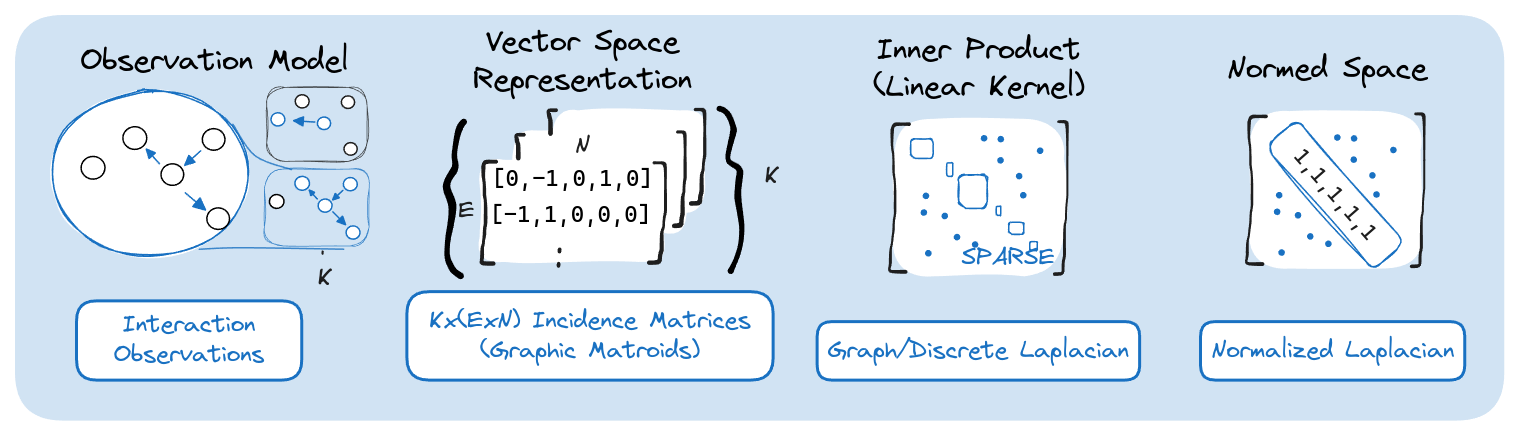
\includegraphics[keepaspectratio]{images/relation-observations.png}}

}

\caption{Edge Relation Observational Model}

\end{figure}%

\chapter{Hypergraphs from Coocurrence
Observations}\label{hypergraphs-from-coocurrence-observations}

\begin{figure}[H]

{\centering \pandocbounded{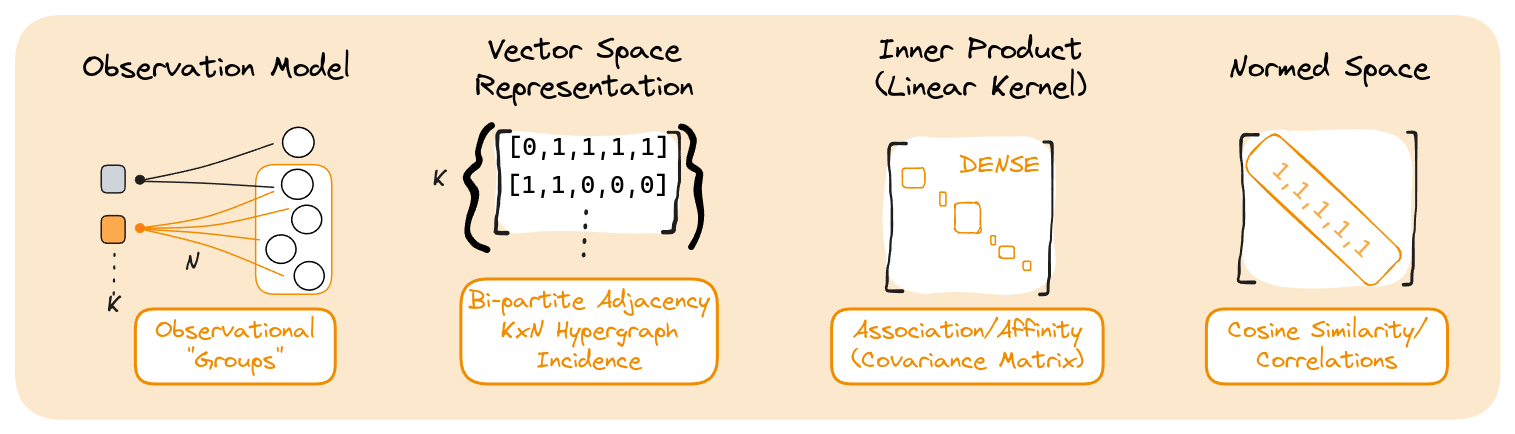
\includegraphics[keepaspectratio]{images/hypergraph-observations.png}}

}

\caption{Hyperedge Relation Observational Model}

\end{figure}%

\chapter{Review: Projections and Inverse
Problems}\label{review-projections-and-inverse-problems}

I.e. trying to ``recover'' one from the other. In a way, proceduralizing
the precautions described in \textcite{WhyHowWhen_Torres2021}.

\begin{quote}
Takeaway: a way to organize existing algorithms, AND highlight unique
set of problems we set out to solve
\end{quote}

\section{Connecting Graphs \& Hypergraphs as
Adjoint}\label{connecting-graphs-hypergraphs-as-adjoint}

i.e.~Network Recovery as an Inverse Problem

\begin{figure}[H]

{\centering \pandocbounded{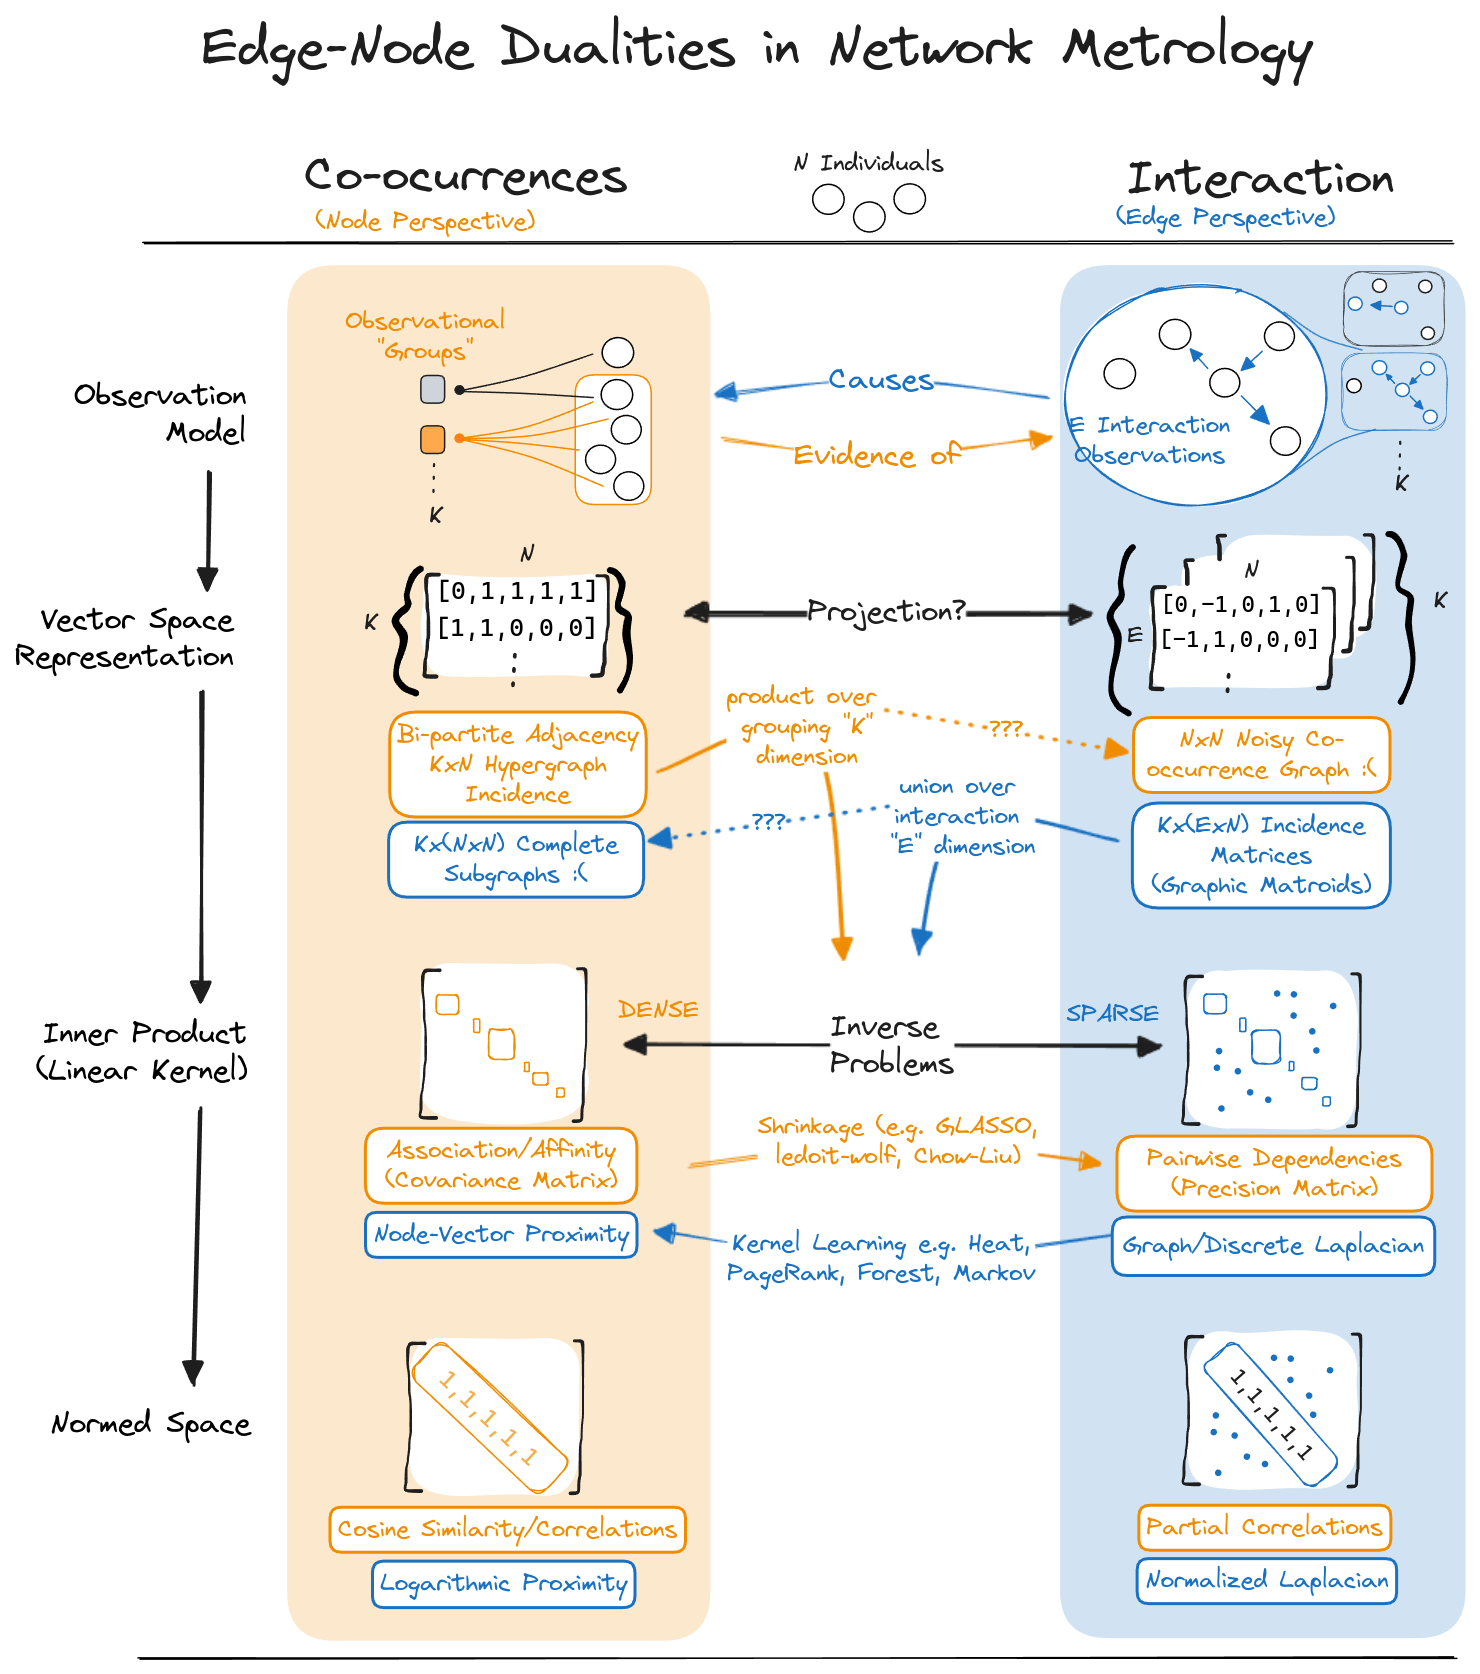
\includegraphics[keepaspectratio]{images/adjoint-cheatsheet.png}}

}

\caption{Relating Graphs and Hypergraph/bipartite structures as adjoint
operators}

\end{figure}%

\section{Algorithmic Information Loss in
Literature}\label{algorithmic-information-loss-in-literature}

\begin{itemize}
\tightlist
\item
  Observation-level loss (starting with the inner product or kernel)
\item
  Non-generative model loss (no projection of data into model space)
\item
  no uncertainty quantification
\end{itemize}

Sorting algorithms\ldots{} \emph{none address all three!}

i.e.~MOTIVATES FOREST PURSUIT

\part{Recovery from Bipartite Occurrence Records}

\chapter{Nonparametric Network Recovery With Random Spanning
Forests}\label{nonparametric-network-recovery-with-random-spanning-forests}

\begin{quote}
filling the gap we saw in the literature
\end{quote}

\section{Generative Model
Specification}\label{generative-model-specification}

\begin{figure}[H]

{\centering \pandocbounded{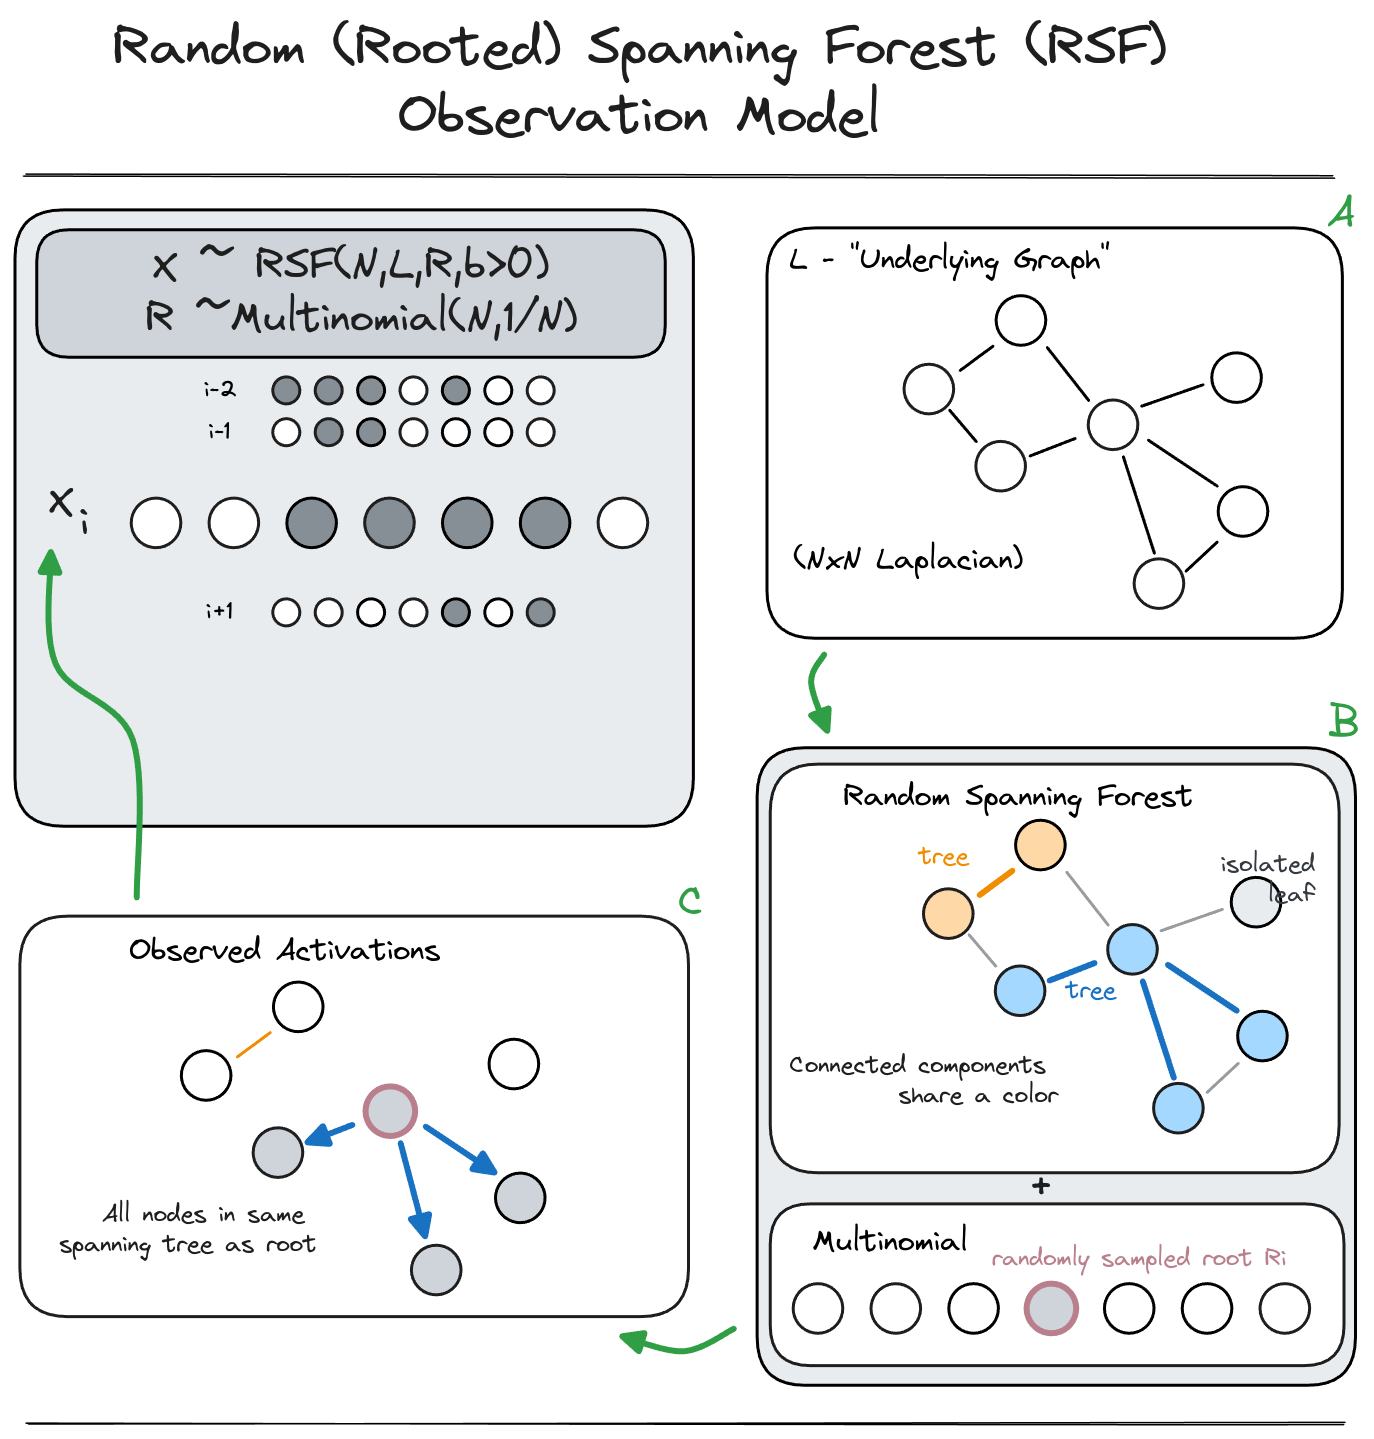
\includegraphics[keepaspectratio]{images/random-spanning-forests.png}}

}

\caption{Explanation of the Random Spanning Forest generative model for
binary activation observations}

\end{figure}%

\section{Forest Pursuit: Approximate Recovery in Near-linear
Time}\label{forest-pursuit-approximate-recovery-in-near-linear-time}

I.e. the PLOS paper (modified basis-pursuit via MSTs)

\section{Bayesian Estimation by Gibbs
Sampling}\label{bayesian-estimation-by-gibbs-sampling}

I.e. the unwritten paper, modifying technique by
\textcite{BayesianSpanningTree_Duan2021} for RSF instead of RSTs

\chapter{LFA: Latent Forest
Allocation}\label{lfa-latent-forest-allocation}

\part{Application and Future Development}

\chapter{Qualitative Application of Relationship
Recovery}\label{qualitative-application-of-relationship-recovery}

\chapter{Recovery from Ordered Random-Walk Observation
Sets}\label{recovery-from-ordered-random-walk-observation-sets}

Like before, but with the added twist of \emph{knowing} our nodes were
activated with a particular partial order.

\emph{insert from
\autocite{OrganizingTaggedKnowledge_Sexton2020,UsingSemanticFluency_Sexton2019}}


\printbibliography



\end{document}
